\section{Introduction}
\label{sec:intro}

A segmentation model that leaves the site where it was trained meets a new scanner, a new protocol or, in nuclear medicine, a new radiotracer.
Its accuracy drops, and the receiving site usually holds a small labelled set with which it could adapt the model.
Adapting is the obvious move, and the computer-vision toolbox for it is rich: fine-tuning, test-time adaptation~\cite{sun2020ttt,wang2021tent,karani2021tta}, self-training~\cite{lee2013pseudo,xie2020noisy}, and, increasingly, agents that critique and repair their own outputs~\cite{madaan2023selfrefine,shinn2023reflexion}.
All of them are judged by an \emph{average}: mean Dice on a validation set.

In medicine the average is not the decision that matters.
An update that raises mean Dice can still delete a metastasis in one patient, and that patient is not consoled by the mean.
Clinicians state the requirement as ``first, do no harm''; regulators increasingly ask that a model's planned changes be specified, with their verification method, before they are made~\cite{fda2023pccp,feng2022monitoring}.
What is missing is a way to make an \emph{update decision} that carries a statement of the form: \emph{this update harms at most a fraction $\delta$ of future patients, and this statement is wrong with probability at most $\alpha$.}

\para{This paper.} We propose \textbf{Certified Self-Improvement} (\ours), a certify-before-deploy protocol for updating a deployed segmentation system (\cref{fig:overview}).
Candidate updates are built on an adaptation set $\A$.
Each candidate defines a null hypothesis ``its patient-level harm rate exceeds $\delta$'', which is tested on a disjoint certification set $\B$ with the Learn-then-Test (LTT) framework~\cite{angelopoulos2021ltt}; a candidate is deployed only if its hypothesis is rejected, and otherwise the system \emph{rolls back} to what is already deployed.
Harm is defined per patient and relative to the deployed system---a lesion that was detected and is no longer, or a Dice drop larger than $0.01$---so the guarantee speaks to exactly the event a clinician fears.
The protocol is agnostic to what the update is: we apply it both to a learned \emph{refinement agent} that edits the segmenter's output and to the \emph{segmenter's weights}.

\para{Testbed.} We transfer an FDG PET/CT tumour-segmentation system~\cite{gatidis2022autopet} to PSMA PET/CT, a different tracer with different physiological uptake, on 377 patients split into adaptation, certification and locked test sets (126/126/125).
Every analysis was pre-registered and every test arm was hash-locked before the test set was read, once.

\para{Findings.}
\textbf{(i)} Zero-shot, the system is safe but poor: Dice $0.11$ and over $700$\,mL of false-positive volume per scan.
\textbf{(ii)} Certified updates of the refinement agent are safe (0 of 125 test patients harmed) but small ($+0.009$ Dice): an agent that edits a poor segmentation cannot create a good one.
\textbf{(iii)} Certified fine-tuning of the segmenter lifts Dice from $0.11$ to $0.55$ and cuts false-positive volume by $98\%$ on the locked test.
At our pre-registered tolerance $\delta=5\%$ the certificate \emph{refused} this switch---4 of 126 certification patients were harmed---and at $\delta=10\%$ it accepted it; on the locked test 2.4\% of patients were harmed (95\% upper bound 6.1\%).
\textbf{(iv)} Without the certificate, the same machinery is dangerous: naive self-improvement harms 11 test patients and loses 20 lesion detections, pseudo-label self-training harms 4 with no gain, and over 1,000 resampled splits naive selection breaks a 5\% harm promise in $98.5$--$99.6\%$ of splits, against $0.2$--$0.5\%$ for \ours, on three segmentation backbones.

\para{Contributions.}
\begin{enumerate}[nosep,leftmargin=*]
\item A certify-before-deploy formulation of self-improvement for segmentation, with a \emph{patient-level, relative} harm risk and a finite-sample guarantee (\cref{sec:method}).
\item A pre-registered, locked study of self-improvement under a real clinical domain shift, at two levels---agent and segmenter---with naive, pseudo-label and uncalibrated baselines (\cref{sec:setup,sec:results}).
\item Evidence that the guarantee holds where naive selection fails, across three backbones, and where three further rules fail (\cref{sec:validity}); a patient-level analysis showing how averages hide harm (\cref{sec:patients}); and a \emph{risk--benefit dial} with its sample-size cost (\cref{sec:dial}).
\item An honest account of what certification cannot do: it bounds risk, it does not create benefit; the large gain comes from adapting the segmenter, and the guarantee costs samples (\cref{sec:discussion}).
\end{enumerate}

\begin{figure*}[t]
  \centering
  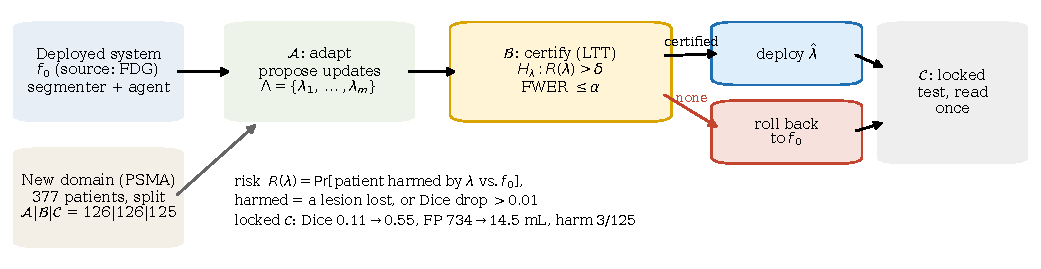
\includegraphics[width=\linewidth]{fig/fig_overview.pdf}
  \caption{\textbf{Certified Self-Improvement.}
  A deployed system $f_0$ meets a new domain.
  Candidate updates $\Lam$ (refinement-agent policies or segmenter weights) are built on the adaptation set $\A$ only.
  On the certification set $\B$, each $\lambda$ is a hypothesis $H_\lambda: R(\lambda)>\delta$, where $R$ is the probability that $\lambda$ harms a patient relative to $f_0$; Learn-then-Test rejects a subset with family-wise error at most $\alpha$.
  The most beneficial certified update is deployed; if none is certified the system rolls back to $f_0$.
  The locked test set $\C$ is read once.
  Numbers: segmenter-level update, PSMA PET/CT, locked $\C$ (\cref{tab:main}).}
  \label{fig:overview}
\end{figure*}
